%% =============================================================================
%% Who Benefits from Cognitive Behavioral Therapy?
%% Generic Machine Learning Inference on Heterogeneous Treatment Effects
%% Applied to Blattman, Jamison & Sheridan (2017)
%% =============================================================================

\documentclass[11pt]{article}

\usepackage[margin=0.5in]{geometry}
\usepackage{amsmath,amssymb}
\usepackage{graphicx}
\usepackage{booktabs}
\usepackage{natbib}
\usepackage{hyperref}
\usepackage{setspace}
\usepackage{caption}
\usepackage{subcaption}
\usepackage{float}
\usepackage{array}
\usepackage{lscape}

\hypersetup{colorlinks=true, citecolor=blue, linkcolor=blue, urlcolor=blue}
\doublespacing

\title{\textbf{Who Benefits from Cognitive Behavioral Therapy?} \\
\large Generic Machine Learning Inference on Heterogeneous Treatment Effects \\
in a Crime-Reduction Experiment in Liberia}

\author{Jovitah Namutebi and Pedro Ferreira \\ \small ECON 2148: Causal Inference in Economics} %\\ \small Harvard University}

\date{May 2026}

%\thispagestyle{empty}

\begin{document}

\maketitle

%% =============================================================================
\section{Introduction}
%% =============================================================================

In our empirical work, we have personally struggled with the question of studying heterogeneous treatment effects. Conventional approaches usually prescribe pre-specifying a small number of subgroups based on theory or prior evidence, and then testing for differences in treatment effects across these subgroups. Though pre-specification can alleviate concerns about data mining and multiple hypothesis testing, it is still difficult to know in advance which characteristics will be the most relevant moderators of treatment response, especially when rich baseline data is available.
Knowing \textit{who} benefits most from an intervention is crucial for policy design and should also inform our understanding of economics.

In this essay, we try to maneuver this challenge by applying the Generic Machine Learning (Generic ML) framework of \citet{chernozhukov2025}, which is relevant for the work of the both of us.
\citet{chernozhukov2025} propose an agnostic, machine-learning-based approach
that sidesteps the problems highlighted above by targeting coarser but tractable
objects: the Best Linear Predictor of the Conditional Average Treatment Effect (CATE) on an ML proxy, the Sorted
Group Average Treatment Effects (GATES), and the Classification Analysis
(CLAN). By using repeated sample-splitting and quantile aggregation, their
method achieves valid inference under weak assumptions, without requiring the
ML estimator to be consistent.

We apply this framework to \citet{blattman2017}'s randomized
experiment, which assigned 999 high-risk men in Monrovia, Liberia, to a
$2\times 2$ factorial design crossing an eight-week cognitive behavioral
therapy (CBT) program with a \$200 cash grant. The experiment is
particularly well-suited for Generic ML for three reasons. First, the replication package includes 57
baseline covariates covering demographics, economic status, mental health,
personality, time preferences, and criminal history, which can be considered as potential
moderators. Second, the randomization was conducted at the individual level,
avoiding the small-cluster problem that hampers Generic ML applications to
many field experiments. Third, the sample of $N = 999$ -- while
modest by ML standards -- is among the largest in the literature among trials with individual-level randomization, as far as we know.\footnote{We considered applying the method to other much larger-scale RCTs, like \cite{banerjee2023electronic}, which comprise virtually millions of individuals. But these are often clustered randomized trials, with no more than hundreds of clusters.}
On top of the methodological convenience, there are two other reasons that make this exercise intellectually interesting. First, a relevant policy question is whether expensive behavioral interventions such as CBT should be universally provided or targeted toward individuals predicted to benefit most. Generic ML provides a natural framework for evaluating whether baseline covariates contain sufficient information to support such targeting. Second, the question of heterogeneity in CBT effects is still open. \cite{blattman2017} did not pre-specify any heterogeneity analysis, and explicitly did not explore heterogeneity in CBT effects because of that.

We find new results. Using the full factorial sample to maximize power, we find evidence of statistically significant heterogeneity in long-run treatment effects ($\hat\beta_2 = 0.557$, $p = 0.060$). The CLAN then characterizes what distinguishes the men at the top of that ranking. A natural prior would be that CBT works best for ``marginal'' criminals -- those with stronger family ties, more social support, lower criminal embeddedness (who face fewer barriers to adopting a prosocial identity). The data suggest the opposite. The men who sustain the largest long-run reductions in antisocial behavior were, at baseline, the most impulsive, the most criminally active, the most psychologically distressed, and the most economically precarious. %Far from reaching those closest to the margin, CBT's lasting impact concentrates among those deepest in crisis --- those for whom the program's identity-transformation mechanism represented the most consequential shift.

The essay proceeds as follows. Section~\ref{sec:blattman} reviews the
experimental context. Section~\ref{sec:method} describes the Generic ML
methodology. Section~\ref{sec:setup} describes the empirical setup.
Section~\ref{sec:results} presents and interprets the results.
Section~\ref{sec:conclusion} concludes.

%% =============================================================================
\section{Experimental Context}
\label{sec:blattman}
%% =============================================================================

\citet{blattman2017} recruited 999 criminally active men in Monrovia, Liberia,
aged 18--35, through a targeted street-recruitment process in five high-crime
neighborhoods. The sample represents the highest-risk segment of the
population: men engaged in drug-selling, theft, and interpersonal violence who
would ordinarily be excluded from development programs.

The study used a $2\times 2$ factorial design. In a first lottery, men were
assigned to receive or not receive an offer of a CBT program (the Sustainable Transformation
of Youth in Liberia, STYL). In a second, independent lottery, men
were assigned to receive or not receive a unconditional \$200 cash grant. This produced four
experimental arms: therapy-only (28\%), cash-only (25\%), therapy-plus-cash
(25\%), and pure control (22\%).

\paragraph{The CBT intervention.}
STYL was an eight-week group-based CBT program run by the Network for
Empowerment and Progressive Initiatives (NEPI). The curriculum combined
psychotherapeutic techniques from two complementary mechanisms. First, it
aimed to build self-regulation and patience: facilitators taught men to manage
anger, resist impulse, and develop a future-oriented mindset. Second, it
promoted a noncriminal social identity: facilitators encouraged men to
re-identify with mainstream society, visit banks and markets, and adopt
prosocial behaviors. Nearly two-thirds of enrolled men completed the
eight-week program.

\paragraph{The cash grant.}
A separate organization distributed \$200 (roughly three months' wages)
unconditionally, about three months after therapy ended. The grant was
designed as a complementary test of whether financial resources could
consolidate the behavioral changes initiated by therapy.

\paragraph{Main findings.}
\citet{blattman2017} report large short-term effects of both therapy and cash
on antisocial behavior, with therapy alone reducing a standardized antisocial behavior
index by roughly 0.20 standard deviations five weeks after treatment. At the
twelve-month follow-up, however, only the therapy-plus-cash arm maintains
significant reductions in antisocial behavior. The authors hypothesize that cash allowed men
to  practice the self-control skills acquired in therapy by providing
capital for legal self-employment, thereby reinforcing behavior change through
learning-by-doing.

%% =============================================================================
\section{Generic ML: Quick Overview}
\label{sec:method}
%% =============================================================================

We now quickly describe the Generic ML framework following \citet{chernozhukov2025}.
The setting is a randomized experiment with $N$ i.i.d.~observations
$(Y_i, D_i, Z_i)$, where $Y_i$ is the outcome, $D_i \in \{0,1\}$ is the
binary treatment indicator, and $Z_i$ is a (possibly high-dimensional) vector
of baseline covariates. The propensity score is known: $p(Z_i) =
\Pr(D_i=1\,|\,Z_i)$.

The CATE is the central object of interest:
\[
s_0(z) \;:=\; \mathbb{E}[Y(1) - Y(0) \,|\, Z=z],
\]
where $Y(1)$ and $Y(0)$ are potential outcomes. In a randomized experiment,
$D \perp (Y(1),Y(0)) \,|\, Z$, so $s_0(z)$ is identified by
\[
s_0(z) = \mathbb{E}[Y\,|\,D=1,Z=z] - \mathbb{E}[Y\,|\,D=0,Z=z].
\]
Because $Z$ may be high-dimensional and $s_0$ can be a complex nonlinear
function, direct nonparametric estimation of $s_0$ is subject to the curse of
dimensionality and, for generic ML estimators, may not converge consistently. \citet{chernozhukov2025} take an agnostic view: they do not
require the ML estimator $S(Z)$ to converge to $s_0(Z)$, and instead build
valid inference on coarser features of the CATE.

The approach relies on random sample splitting. The data are
partitioned into a main sample $M$ (used for inference) and an auxiliary
sample $A$ (used for ML training). In Stage 1, an ML method is applied to $A$
to produce a proxy predictor $S(Z)$ for the CATE. In Stage 2, $S(Z)$ is used
in the main sample to estimate three targets.

To address the randomness of the split, the procedure is repeated over $K$
random splits (here $K=100$) and results are aggregated via quantile
aggregation.
Confidence
intervals are the median of split-specific confidence bands.
\citet{chernozhukov2025} show that quantile aggregation yields lower
estimation risk than a single split.

\subsection{Best Linear Predictor (BLP)}
The BLP regresses the outcome $Y$ on the proxy $S(Z_i)$ in the main sample,
using a modified regression that leverages the Riesz representation:
\[
Y_i \;=\; \alpha_0 + \alpha_1 D_i + \underbrace{\beta_1}_{=\,\text{ATE}} (D_i - p_i) + \underbrace{\beta_2}_{=\,\text{HET}} (D_i - p_i)[S(Z_i) - \bar S] + \varepsilon_i,
\]
where $p_i = p(Z_i)$ is the propensity score and $\bar S$ is the mean of
$S(Z_i)$ in the sample. The coefficient $\beta_1$ is a valid estimator of the
ATE under weak conditions. Crucially, $\beta_2 > 0$ is the coefficient on the
interaction $(D_i-p_i)[S(Z_i)-\bar{S}]$: if the ML proxy contains genuine
information about the CATE, then $\beta_2 > 0$. A test of $H_0:\beta_2=0$
is thus a test for whether there is any detectable heterogeneity in treatment effects on the covariates
that can be predicted by the ML proxy.

The key theoretical object in the empirical analysis is the BLP coefficient on the interaction between treatment assignment and the ML proxy. Because of this, we include a more formal statement of the BLP result here.

\textbf{Proposition 1.} \textit{Suppose treatment is randomly assigned with known propensity score
$p(Z)=P(D=1\mid Z)$, where $0<p(Z)<1$. Let
\[
s_0(Z)=E[Y(1)-Y(0)\mid Z]
\]
denote the conditional average treatment effect, and let $S(Z)$ be a fixed proxy for $s_0(Z)$ obtained from the auxiliary sample. If $\mathrm{Var}(S(Z))>0$, then the coefficient $\beta_2$ in the population best linear predictor
\[
BLP[s_0(Z)\mid S(Z)]
=
\beta_1+\beta_2(S(Z)-E[S(Z)])
\]
is given by
\[
\beta_2=
\frac{\mathrm{Cov}(s_0(Z),S(Z))}{\mathrm{Var}(S(Z))}.
\]
Thus, $\beta_2$ measures whether the ML proxy ranks individuals according to true treatment-effect heterogeneity. If $\beta_2=0$, then the proxy contains no linear predictive information about the CATE.}

Proof. See Appendix A.

\subsection{Sorted Group Average Treatment Effects (GATES)}

GATES sorts individuals into $K$ groups based on their predicted CATE
$S(Z_i)$, from the lowest ($k=1$, least affected) to the highest ($k=K$,
most affected). The group average treatment effects $\gamma_k =
\mathbb{E}[s_0(Z)\,|\,G_k]$ are estimated via an auxiliary regression in the
main sample. The GATES answer the question:Is the treatment
heterogeneous, and in what direction? The contrast $\gamma_4 - \gamma_1$
tests whether the most and least affected groups have different average
treatment effects.

\subsection{Classification Analysis (CLAN)}

CLAN characterizes the most and least affected groups using observable
characteristics. For each baseline covariate $W_j$, CLAN estimates the
average of $W_j$ in each GATES group $G_k$. The contrast $\delta_4^j -
\delta_1^j = \mathbb{E}[W_j\,|\,G_4] - \mathbb{E}[W_j\,|\,G_1]$ identifies
which observable characteristics are associated with being most (vs.~least)
responsive to treatment. Inference on $\delta_4^j - \delta_1^j$ is valid
without multiple-testing correction within each variable, though interpretation
across many variables should be cautious.

%% =============================================================================
\section{Empirical Setup}
We now implement the BLP, GATES, and CLAN estimators described above in the context of Blattman et al. (2017), focusing on the antisocial behavior index and the number of thefts as primary outcomes.
\label{sec:setup}
%% =============================================================================

\subsection{Treatment Indicators and Outcomes}

Because Generic ML requires a binary treatment, we organize our six analyses in two blocks. The first block (A1 through A3) compares the pure CBT treatment arm against the pure control group on three outcomes, short-term and long-term antisocial behavior and short-term thefts. The second block (A4 through A6) exploits the full $2\times 2$ factorial design, pooling both CBT arms as treated ($D=1$) and both non-CBT arms -- pure control and cash-only -- as control ($D=0$), focusing on the same three outcomes. This factorial main-effect estimator uses all $N= 999$ observations in round 1 (or the full long-term sample in A5), roughly doubling the effective sample size relative to A1 through A3 and substantially increasing power for the heterogeneity test. Table \ref{tab:analyses} summarizes the six analyses.

\begin{table}[H]
\centering
\caption{Summary of analyses}
\label{tab:analyses}
\begin{tabular}{llll}
\toprule
Label & Treatment ($D=1$) & Outcome ($Y$) & $N$ \\
\midrule
A1 & CBT only vs. control & Antisocial behavior index (short-term) & 463 \\
A2 & CBT only vs. control & Antisocial behavior index (long-term)  & 468 \\
A3 & CBT only vs. control & Number of thefts (short-term)           & 463 \\
\midrule
A4 & CBT (any) vs. cash+control & Antisocial behavior index (short-term) &  922 \\
A5 & CBT (any) vs. cash+control & Antisocial behavior index (long-term)  & 947 \\
A6 & CBT (any) vs. cash+control & Number of thefts (short-term)           & 922 \\
\bottomrule
\end{tabular}
\begin{minipage}
{\textwidth}
\footnotesize \noindent\textit{Note.} In A4--A6, treatment is assigned to any man offered CBT (either CBT-only or CBT+cash); control comprises cash-only and pure-control men. This is the main-effect contrast in a $2\times 2$ factorial design, averaging over cash assignment, which is orthogonal to CBT assignment by construction.
\end{minipage}
\end{table}



The primary outcome in analyses A1, A2, A4, and A5 is the standardized antisocial behavior
index, a composite of stealing, fighting,
carrying weapons, drug selling, and hostility. Higher values indicate more
antisocial behavior. The short-term outcome is measured approximately five
weeks after treatment (round 1 of the panel) while the long-term outcome is
measured twelve to thirteen months after treatment (round 5).

Analyses A3 and A6 examine a secondary outcome: the number of thefts committed
in the past two weeks. This captures the behavioral outcome most directly
linked to crime reduction. We second the discussion around measurement errors and reporting bias to \cite{blattman2017}.

\subsection{Covariates}

The matrix $Z$ includes all 57 baseline covariates from Blattman's
balance table (Table 1 of their paper), all available in their replication package. These include:

\begin{itemize}
\item \textbf{Demographics}: age, marital status, number of children,
  schooling, literacy, health, disability.
\item \textbf{Mental health}: depression and distress scores.
\item \textbf{Conflict exposure}: war experience, faction membership,
  ties to military commanders.
\item \textbf{Economic situation}: weekly earnings, wealth index,
  homelessness, savings, debt.
\item \textbf{Labor market}: hours in illicit, agricultural, wage, and
  high-skill work.
\item \textbf{Substance use}: drug selling, alcohol use, marijuana use,
  hard drug use.
\item \textbf{Criminal history}: number of thefts (violent and non-violent),
  disputes, hostility.
\item \textbf{Noncognitive skills}: conscientiousness, neuroticism, grit,
  reward responsiveness, locus of control, impulsivity, self-esteem.
\item \textbf{Preferences}: patience (incentivized game and declared),
  risk aversion, time inconsistency.
\item \textbf{Cognitive ability}: cognitive test score, executive function.
\end{itemize}

Missing values in $Z$ (present for a small share of observations) are imputed
using column medians. The CLAN is performed on a subset of 19 covariates
selected for interpretability.

\subsection{Implementation}

We use the GenericML R package \citep{welz2022}, which implements the
\citet{chernozhukov2025} methodology. We set $K=100$ random splits, with
auxiliary proportion 50\%, and use 90\% confidence intervals throughout. The propensity score is set to constant equal to the sample mean of $D$ (given it is an RCT). Analyses A1, A3 use
short-term data (round 1), restricted to the CBT-only arm versus pure control. Analysis A2 uses long-term data (round 5), CBT-only versus pure control. Analyses A4 and A6 use the full round-1 sample ($N= 999$) with the factorial treatment indicator. Analysis A5 uses the full round-5 sample.

%% =============================================================================
\section{Results}
\label{sec:results}
%% =============================================================================

%% =============================================================================

\subsection{Best Linear Predictor: Average Effects and Heterogeneity}

\begin{table}[H]
\centering
\caption{Best Linear Predictor results}
\label{tab:blp}
\resizebox{\textwidth}{!}{
\begin{tabular}{lcccccc}
\toprule
& \multicolumn{3}{c}{$\hat\beta_1$ (ATE)} &
  \multicolumn{3}{c}{$\hat\beta_2$ (Heterogeneity)} \\
\cmidrule(lr){2-4}\cmidrule(lr){5-7}
Analysis & Estimate & 90\% CI & $p$-value
         & Estimate & 90\% CI & $p$-value \\
\midrule
A1: CBT only, ST ASB & $-0.225$ & $[-0.473,\ 0.022]$ & 0.073 & $\phantom{-}0.146$ & $[-0.339,\ 0.654]$ & 0.556 \\
A2: CBT only, LT ASB & $-0.010$ & $[-0.250,\ 0.227]$ & 0.931 & $-0.244$ & $[-1.258,\ 0.763]$ & 0.673 \\
A3: CBT only, ST Theft & $-0.934$ & $[-2.078,\ 0.223]$ & 0.109 & $\phantom{-}0.271$ & $[-0.210,\ 0.861]$ & 0.198 \\
\midrule
A4: CBT (any), ST ASB & $-0.218$ & $[-0.382,{-0.054}]$ & 0.009 & $\phantom{-}0.282$ & $[-0.158,\ 0.735]$ & 0.201 \\
A5: CBT (any), LT ASB & $-0.176$ & $[-0.334,{-0.013}]$ & 0.034 & $\phantom{-}0.557$ & $[-0.028,\ 1.130]$ & 0.060 \\
A6: CBT (any), ST Theft & $-0.649$ & $[-1.338,\ 0.081]$ & 0.078 & $-0.065$ & $[-0.654,\ 0.493]$ & 0.819 \\
\bottomrule
\end{tabular}
}
\begin{minipage}{\textwidth}
\footnotesize \textit{Notes:} Median estimates and 90\% confidence intervals over 100 random sample splits. $\hat\beta_1$ estimates the ATE; $\hat\beta_2$ tests $H_0$: no heterogeneity. Best learner by BLP criterion: A1: lasso; A2: random forest; A3: lasso; A4: lasso; A5: random forest; A6: lasso. Outcome for A1, A2, A4, A5: standardized antisocial behavior index (lower = more prosocial). A3, A6: number of thefts in the past two weeks. A4--A6 use the full $2\times2$ factorial design (any CBT vs.\ cash + control).
\end{minipage}

\end{table}

\paragraph{Average effects ($\hat\beta_1$).}
The BLP results paint a coherent picture across the two blocks of analyses and are broadly consistent with Blattman's ITT estimates. In the narrow comparisons (A1 through A3), CBT alone reduces the standardized antisocial behavior index in the short run ($\hat\beta_1 = -0.225$, $p = 0.073$), but this effect appears to dissipate by the twelve-month follow-up ($\hat\beta_1 = -0.010$, $p = 0.931$). The effect on the number of thefts is negative and large in magnitude ($\hat\beta_1 = -0.934$) but imprecisely estimated ($p = 0.109$), consistent with high variance in self-reported theft counts.

The factorial main-effect analyses (A4 through A6) confirm and considerably sharpen these findings. Using all $N\approx 999$ observations, the estimated CBT effect on short-term antisocial behavior becomes the most precisely estimated result in the table: $\hat\beta_1 = -0.218$ ($p = 0.009$). %This is the main payoff of the factorial design: by recovering the marginal effect of CBT averaging over cash assignment--which is orthogonal to CBT by construction--we nearly double the effective sample and obtain a highly significant average effect.
By recovering the marginal effect of CBT averaging over cash assignment (which is orthogonal to CBT by construction), the design doubles the sample and yields a highly significant average effect.
The similarity of the point estimates in A1 ($-0.225$) and A4 ($-0.218$) suggests that cash assignment does not substantially confound the CBT main effect, as expected from independent randomization.

The factorial design also rescues the long-term finding. In A2, where only CBT-only participants are compared to control ($N = 463$), the twelve-month effect on antisocial behavior is essentially zero ($\hat\beta_1 = -0.010$, $p = 0.931$). In A5, which uses the full factorial sample ($N= 950$), the long-term average effect is $\hat\beta_1 = -0.176$ ($p = 0.034$) -- negative, meaningful, and statistically significant. This suggests that the apparent fade-out of CBT effects visible in the narrow comparison could be partly an artifact of limited power. The factorial effect on short-term theft (A6) is also negative ($\hat\beta_1 = -0.649$, $p = 0.078$), marginally significant and consistent with A3.

\paragraph{Heterogeneity ($\hat\beta_2$).}
%The pattern of $\hat\beta_2$ estimates reveals an important asymmetry across outcomes and time horizons. For short-term antisocial behavior, $\hat\beta_2$ is positive in both the narrow (A1: $0.146$, $p = 0.556$) and factorial (A4: $0.282$, $p = 0.201$) comparisons, and the progression toward lower $p$-values as the sample grows is consistent with a modest true signal below the detection threshold of the smaller design. For theft, the estimates are positive in the narrow comparison (A3: $0.271$, $p = 0.198$) but near zero in the factorial (A6: $-0.065$, $p = 0.819$), offering no evidence of treatment effect heterogeneity on that margin.
The test cannot reject the null of no heterogeneity in any of the narrow comparisons (A1 through A3). The absence of detectable heterogeneity in A1 through A3 does not imply that treatment effects are uniform. \citet{chernozhukov2025} note that the power of the BLP test may be limited when true heterogeneity is modest. 

However, exploiting the larger sample size of factorial design, the test can reject the null of no heterogeneity in one of the three factorial analyses (A4 through A6). In particular,
the most striking result is in A5: the factorial estimate of $\hat\beta_2$ for long-term antisocial behavior is $0.557$ ($p = 0.060$), statistically significant at the 10\% level. This is the only analysis in which Generic ML can reliably predict -- from baseline characteristics alone -- who benefits most from CBT. The finding has a natural interpretation: while the program shifts the average for most participants in the short run, long-run maintenance of prosocial gains is more selective, concentrated among men whose baseline profiles make them particularly receptive to sustained behavior change. We explore the correlates of this heterogeneity in the GATES and CLAN analyses below.

%In contrast, $\hat\beta_2$ for A2 (CBT only, long-term) is negative ($-0.244$, $p = 0.673$) and insignificant, consistent with the near-zero average effect and low precision in that smaller sample. The emergence of significant heterogeneity in A5 but not A2, for the same outcome, underscores a recurring theme: the factorial design provides the power needed to detect patterns that are simply invisible in the narrower arm-by-arm comparison.

%The absence of detectable heterogeneity in A1 through A3 does not imply that treatment effects are uniform. \citet{chernozhukov2025} note that the power of the BLP test may be limited when true heterogeneity is modest. % Below we show that the GATES and CLAN analyses reveal suggestive distributional patterns even where $\hat\beta_2$ falls short of significance.

\subsection{Sorted Group Average Treatment Effects (GATES)}

We focus the GATES analysis on A5, the analysis that yields significant heterogeneity. Figure~\ref{fig:gates_a5} plots the four group-average treatment effects for the long-term factorial analysis. Individuals are sorted into quartiles based on the lasso's predicted CATE: G1 has the lowest predicted CATE (and hence the largest actual long-run \textit{reduction} in antisocial behavior) and G4 has the highest predicted CATE (smallest actual reduction). Since treatment reduces antisocial behavior, a more negative $\gamma_k$ is a larger beneficial effect.

\begin{figure}[H]
\centering
\caption{Sorted Group Average Treatment Effects (GATES): CBT (any) vs.\ cash+control, long-term antisocial behavior (A5, $N= 947$)}
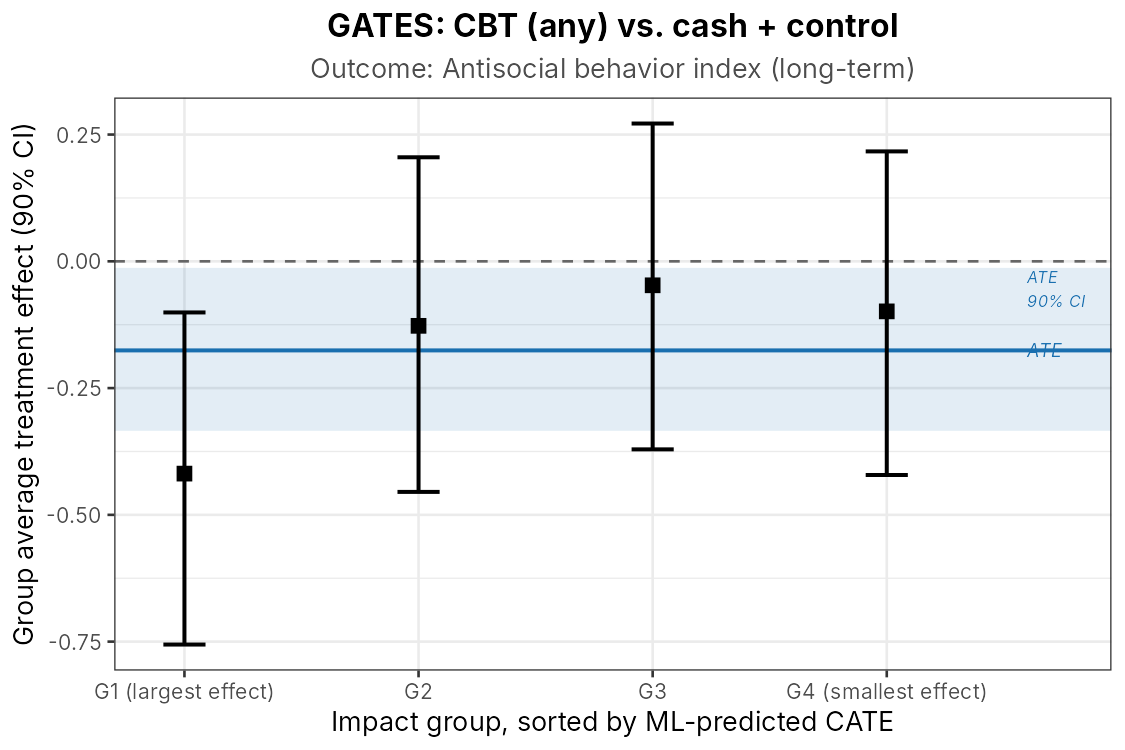
\includegraphics[width=0.7\textwidth]{../Output/GATES_A5.png}
\begin{minipage}
{\textwidth}
\footnotesize \noindent\textit{Note.} Point estimates are medians across 100 splits; bars are 90\% confidence intervals.
  G1 = group with lowest ML-predicted CATE (largest actual effect); G4 = group with highest ML-predicted CATE (smallest actual effect).
\end{minipage}
\label{fig:gates_a5}
\end{figure}

G1 shows the largest and most precisely estimated treatment effect: $\gamma_1 = -0.419$ ($p = 0.010$). Groups G2 through G4 are smaller in magnitude and statistically insignificant ($\gamma_2 = -0.127$, $\gamma_3 = -0.047$, $\gamma_4 = -0.099$). The contrast $\gamma_4 - \gamma_1 = 0.350$ ($p = 0.135$) is positive and relatively large, consistent with the significant $\hat\beta_2 = 0.557$ ($p = 0.060$) from the BLP.

The pattern is coherent with $\hat\beta_2 > 0$ for a negative-direction outcome: a positive $\hat\beta_2$ means higher predicted CATE corresponds to a \emph{less negative} actual effect. The  men that experience smaller long-run reductions are placed  in G4. G1 -- with the lowest predicted CATE -- concentrates the men with the deepest actual reductions. The spread of effects across the four quartiles ($\gamma_4 - \gamma_1 = 0.350$) quantifies how much the treatment effect varies across the CATE distribution.

\subsection{Classification Analysis (CLAN)}

Because $\hat\beta_2$ is statistically significant in A5, the CLAN for the long-term factorial analysis provides a genuine characterization of who benefits most from CBT in the long run. We focus on A5 as the primary CLAN analysis.

\begin{figure}[H]
\centering
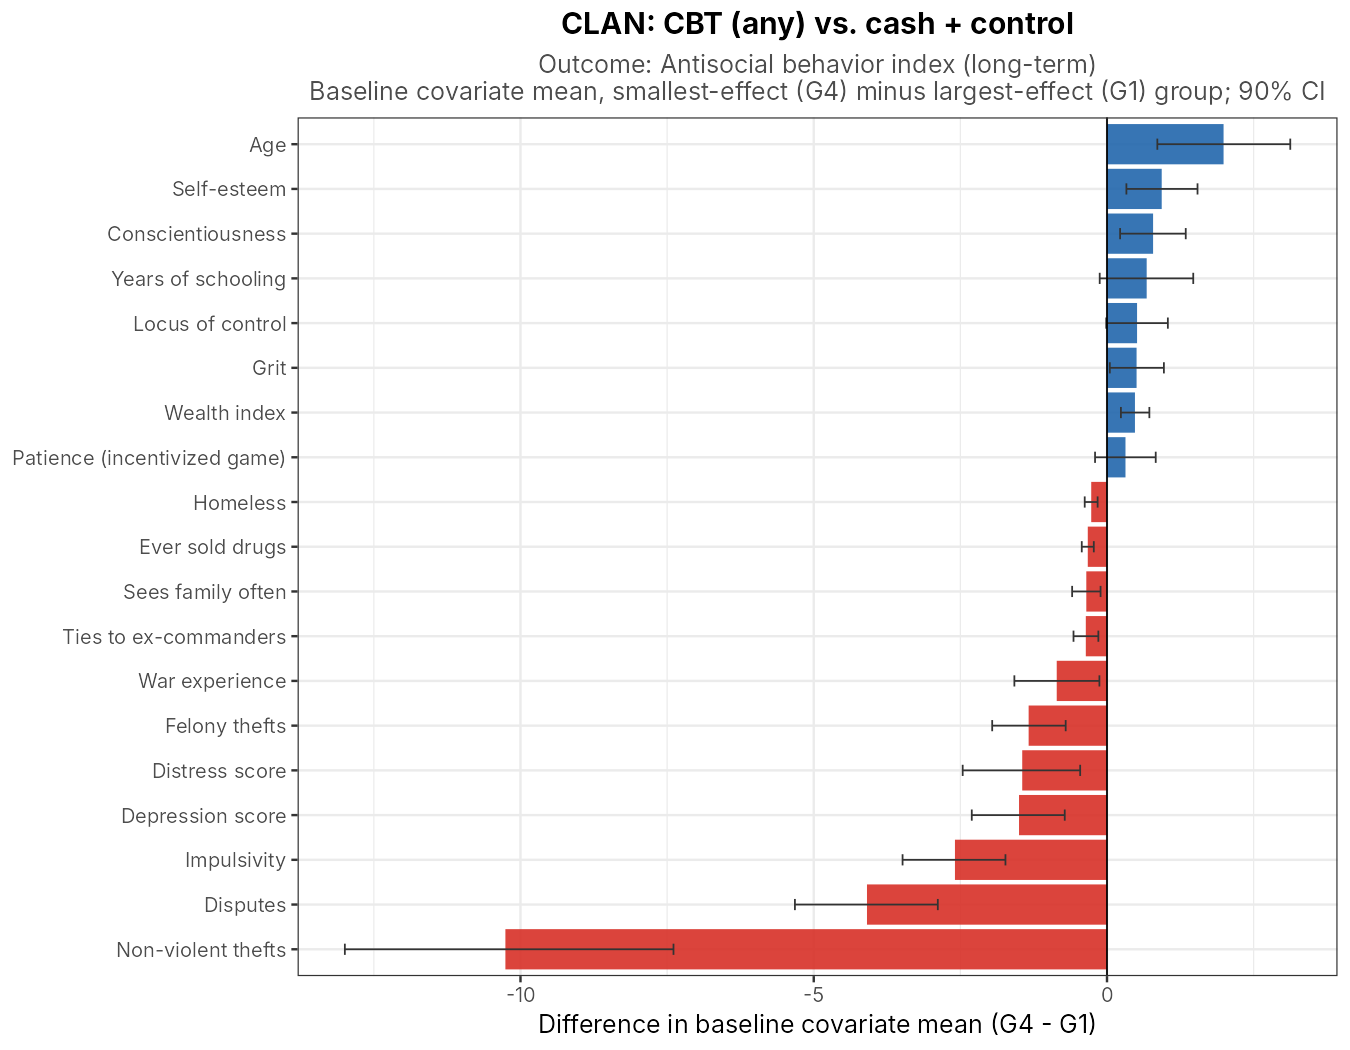
\includegraphics[width=0.85\textwidth]{../Output/CLAN_A5.png}
\caption{CLAN: CBT (any) vs.\ cash+control, long-term antisocial behavior (A5). Each bar shows the
  difference in covariate means between the smallest-effect group (G4, highest predicted CATE)
  and the largest-effect group (G1, lowest predicted CATE), aggregated as medians over 100
  splits (lasso best learner). Positive bars indicate G4 scores higher on that variable;
  negative bars indicate G1 scores higher.}
\label{fig:clan_a5}
\end{figure}

The contrasts in Figure~\ref{fig:clan_a5} reveal a sharp and internally consistent profile. The bars show G4 minus G1: positive values mean the smallest-effect group (G4) scores higher; negative values mean the largest-effect group (G1) scores higher. Several contrasts are large and highly significant:

\begin{itemize}
\item \textbf{Impulsivity}: The smallest-effect group (G4) is $2.59$ points \emph{less} impulsive than the largest-effect group (G1) ($\delta_4 - \delta_1 = -2.59$, $p < 0.001$) -- the largest contrast in absolute terms. Men with high baseline impulsivity, precisely the psychological profile CBT targets, sustain the largest long-run reductions.

\item \textbf{Criminal embeddedness}: G4 reports $10.3$ fewer non-violent thefts ($p < 0.001$), $1.3$ fewer felony thefts ($p < 0.001$), $4.1$ fewer disputes ($p < 0.001$), and is $0.33$ less likely to have ever sold drugs ($p < 0.001$). G4 also had less war experience ($-0.86$, $p = 0.017$) and fewer ties to military commanders ($-0.36$, $p = 0.001$). The largest-effect group (G1) was the most criminally active at baseline.

\item \textbf{Psychological distress}: G4 scores $1.5$ points lower on depression ($p < 0.001$) and $1.45$ points lower on psychological distress ($p = 0.006$). The largest-effect group (G1) entered the program more psychologically distressed.

\item \textbf{Economic precarity}: G4 has a higher wealth index ($+0.48$ standard deviations, $p < 0.001$) and is $0.27$ less likely to have been homeless at baseline ($p < 0.001$). The largest-effect group (G1) is poorer and more economically marginalized.

\item \textbf{Self-regulation}: G4 scores $0.79$ points higher on conscientiousness ($p = 0.008$), $0.50$ points higher on grit ($p = 0.031$), and $0.93$ points higher on self-esteem ($p = 0.003$). The largest-effect group (G1) is less self-regulated with lower self-worth at baseline.

\item \textbf{Age}: G4 is on average $2.0$ years older ($p < 0.001$) and sees family $0.35$ fewer days per week ($p = 0.005$).
\end{itemize}

Taken together, the CLAN identifies the men who sustain the largest long-run reductions in antisocial behavior as those who, at baseline, were the most criminally active, the most psychologically distressed, the most impulsive, the least self-regulated, and the most economically precarious. This is the highest-risk stratum of an already high-risk population.

This finding is counterintuitive. A natural prior would predict that men with more internal resources -- lower impulsivity, higher conscientiousness, more stable economic lives -- would be best positioned to internalize and sustain the self-regulation lessons of CBT. Instead, the data suggest that it is the men with the most to gain and the deepest behavioral deficits who maintain the largest changes over twelve months. A plausible mechanism is that CBT's identity-transformation component (reidentifying with mainstream society, building self-efficacy, restructuring peer relationships) is most consequential for men whose criminal identity is most salient. For men already more self-regulated and less criminally embedded, the marginal contribution of an eight-week program is smaller.

%This picture also contrasts with the short-term CLAN (analysis A4). In the short run, the largest-effect group was psychologically distressed and less educated, but \emph{less} criminally embedded: men who were psychologically vulnerable but had not yet fully committed to a criminal career. In the long run, the largest-effect group is both distressed \emph{and} deeply embedded in crime. Together, the two CLAN analyses suggest that CBT's short-run reach is broad --- extending even to the less criminally embedded --- while its long-run impact concentrates among those whose behavioral problems are most severe and whose need for identity reorientation is greatest.

%% =============================================================================
\section{Conclusion}
\label{sec:conclusion}
%% =============================================================================

We have applied the Generic ML framework of \citet{chernozhukov2025} to study who benefits from CBT in \citet{blattman2017}'s  Liberia experiment, organizing six analyses in two blocks: a narrow block (A1--A3) comparing CBT-only against pure control, and a factorial block (A4--A6) exploiting the full $2\times 2$ design to maximize power.

After confirming \citet{blattman2017}'s main findings on average effects, 
the central finding is that long-run treatment effects are heterogeneous. While short-term effects appear relatively uniform, in the long-run factorial analysis, the BLP coefficient $\hat\beta_2$ is positive and large ($0.557$) and we can reject the null of no heterogeneity at the 10\% level ($p = 0.060$).  The CLAN further characterizes the men at the top of the long-run CATE distribution. A natural prior would be that CBT reaches ``marginal'' criminals -- men with stronger family ties, more social support, lower criminal embeddedness -- who face fewer barriers to adopting a prosocial identity and are therefore more likely to sustain behavior change. The data point in the opposite direction. The men sustaining the largest long-run reductions in antisocial behavior were, at baseline, the most impulsive, the most criminally active, the most psychologically distressed, and the most economically precarious -- the highest-risk stratum of an already high-risk population. This suggests that CBT's identity-transformation mechanism is most consequential precisely where criminal identity is most entrenched, and where the program's social reorientation represents the sharpest departure from baseline conditions.

%% =============================================================================
\pagebreak 
\appendix

\section{Proofs}

\subsection{Proof of Proposition 1}

The BLP is defined as the best linear approximation to the conditional average treatment effect using the proxy $S(Z)$. That is, $\beta_1$ and $\beta_2$ solve
\[
\min_{b_1,b_2}
E\left[
s_0(Z)-b_1-b_2(S(Z)-E[S(Z)])
\right]^2.
\]

Let $\tilde S(Z)=S(Z)-E[S(Z)]$. The minimization problem becomes
\[
\min_{b_1,b_2}
E\left[
s_0(Z)-b_1-b_2\tilde S(Z)
\right]^2.
\]

The first-order condition with respect to $b_1$ is
\[
E\left[
s_0(Z)-b_1-b_2\tilde S(Z)
\right]=0.
\]
Since $E[\tilde S(Z)]=0$, this implies
\[
b_1=E[s_0(Z)].
\]

The F.O.C with respect to $b_2$ is
\[
E\left[
\tilde S(Z)\{s_0(Z)-b_1-b_2\tilde S(Z)\}
\right]=0.
\]
Substituting $b_1=E[s_0(Z)]$ gives
\[
E\left[
\tilde S(Z)\{s_0(Z)-E[s_0(Z)]\}
\right]
-
b_2E[\tilde S(Z)^2]
=0.
\]
Therefore,
\[
b_2=
\frac{
E\left[(S(Z)-E[S(Z)])(s_0(Z)-E[s_0(Z)])\right]
}{
E\left[(S(Z)-E[S(Z)])^2\right]
}.
\]
Equivalently,
\[
b_2=
\frac{\mathrm{Cov}(s_0(Z),S(Z))}
{\mathrm{Var}(S(Z))}.
\]

This implies that, the BLP heterogeneity coefficient is the linear projection coefficient of the true CATE on the ML proxy. If this coefficient is zero, then the ML proxy is uncorrelated with the CATE and does not contain linear predictive information about treatment-effect heterogeneity.

\hfill $\blacksquare$

%% =============================================================================
\newpage
\bibliographystyle{aer}
\bibliography{refs}
%% =============================================================================

\end{document}
